\documentclass[a4paper]{article}

\usepackage[utf8]{inputenc}
\usepackage[T1]{fontenc,url}
\usepackage{cite}
\usepackage{hyperref}
\usepackage{amsmath, amssymb}
\usepackage{tikz}
\usepackage{graphicx}
\usepackage{parskip}
\usepackage{lmodern}
\usepackage{algorithm}
\usepackage{algpseudocode}
\usepackage{epigraph}
\usepackage{listings}
\usepackage{float}
\usepackage{amsthm}
\usepackage{changepage}



\begin{document}
\title{FYS4150 -- Project 2}
\author{Joachim Falck Brodin,
        Fredrik Jaibeer Mahal Nordeng,\\ 
        and Endrias Getachew Asgedom}

\maketitle
\begin{abstract}
\noindent
Three physical problems, the buckling beam and quantum dots with one and two electrons, are reformulated as eigenvalue-problems and solved numerically with the Jacobi rotation algorithm. The method and results are compared in terms of computation time and precision with Armadillo's built in $eig\_sym$ function, as a function of different matrix sizes. In each case analytical solutions are awailable fro comparison. We find the method to perform very well in terms of precision for the buckling beam problem (relative error $\sim10^{-11}$), however in the case of the quantum dots we have a loss of precision (giving us relative error $\sim10^{-4}$) due to complication resulting from the way we represent discretely a boundary that in reality approaches infinity. We find the computational time for the Jacobi algorithm goes as $n^2$, where $n$ is the number of grid points (or the matrix size). Compared with Armadillo's inbuilt method Jacobi's algorithm is computationally faster for $n<10$, but for larger matrices Armadillo's function is much faster. The eigenvalues and eigenvectors from the Jacobi algorithm match the corresponding results from Armadillo's function with a high degree of precision. 
\end{abstract}


\newpage
\tableofcontents

\begin{center}
    GitHub repository at \url{https://github.com/endrias34/FYS4150}
\end{center}
%%% MACROS
\newcommand{\half}{\frac{1}{2}}
\newcommand{\dx}{{\Delta x}}
\newcommand{\bigO}{{\mathcal{O}}}

\newpage

\section{Introduction}
In this project we investigate three different physics problems and reformulate them as matrix-vector equations, that in turn can be cast as eigenvalue-problems. We encounter eigenvalue-problems in many fields of physical sciences and engineering. Here, we will first look at a classical-mechanics problem of a buckling beam, see Fig. \ref{fig: buckling beam}. Initially, the two end points of the beam is held fixed and a force is applied at one end of the beam in the direction towards the origin while the other end is held fixed. The differential equation describing the motion of the beam is transformed into an eigenvalue problem after discretizing and approximating the differentiation by second order Taylor expansion. Consequently, the resulting eigenvectors represent the vertical displacement along the beam, while the eigenvalues correspond to the energy, here given by the length of the beam, the material properties, and the applied force.

In the second and third part of the assignment we consider a quantum dot in a three dimensional harmonic oscillator potential with one and two electrons. As the potential is spherically symmetric the Schrodinger equation can be separated into angular and radial contributions. Here, we consider the radial contribution and treat the problem as one-dimensional, as functions of a scaled distances from the origin for a single electron case and scaled distance between the center of the two, for the two electrons. For this problem, the eigenvectors represent the corresponding wavefunctions, when squared it gives the probability density functions of the scaled distances, and the eigenvalues correspond to the energy levels.

We will use the Jacobi rotation algorithm to solve the three different eigenvalue problems specified above. The accuracy of the Jacobi algorithm is assessed by comparing it with the analytical solution and also with Armadillo's built-in eigenvalue problem solver. The computational efficiency of the Jacobi algorithm is analysed in terms of the size of the matrix and the computation time it takes. We also benchmark the run time of Jacobi's rotation algorithm against Armadillo's implementation.

\begin{figure}[H]
  \centering
  \includegraphics[keepaspectratio,height=10cm, width=12cm]{Buckling beam.png}
  \caption{Illustration of the buckling of a beam}
   \label{fig: buckling beam}
\end{figure}


\section{Theory}
In this section we present the problem formulation for the buckling of a beam and quantum dots in a three dimensional harmonic oscillator potential with one and two electrons \cite{hjorten}.

\subsection{The buckling beam as an eigenvalue problem}\label{sec-bm}
\label{section:beam}
A horizontally oriented beam of length $L$ is fixed at both endpoints, as seen in Fig. \ref{fig: buckling beam}. The beam can oscillate in the vertical direction, with the vertical displacement along the horizontal direction, $x$, denoted as $u(x)$, expressed by the differential equation
\begin{equation}\label{eq-beam}
\gamma \frac{d^2 u(x)}{dx^2} = -Fu(x),
\end{equation}
where $\gamma$ is a material constant and $F$ is an applied force. We assume Dirichlet boundary conditions, $u(0) = u(L) = 0$. We define the dimensionless variable
\begin{equation}
\rho = \frac{x}{L},\quad \rho \in [0,1]
\end{equation}
We rewrite Eq. \eqref{eq-beam} as

\begin{equation}
\frac{d^2 u(\rho)}{d\rho^2}  = -\lambda u(\rho),
\end{equation}
where $\lambda = FL^2/\gamma$. We now wish to discretize our equation, and do so along the lines of what we did in Project 1,


\begin{equation}
-\frac{u_{i+1} + u_{i-1} -2u_i}{h^2} = \lambda u_i,
\end{equation}

with step length, $h = \frac{1-0}{N}$,  $i \in \{0,1,2, ..., N\}$.  Again, we can rewrite this as a set of linear equations,
\begin{equation}\label{eq: matrix}
\begin{bmatrix}
d & e & 0 & 0 & 0 & \dots & 0\\
e & d & e & 0 & 0 & \dots & 0\\
0 & e & d & e & 0 & \dots & 0\\
\dots & \dots & \dots & \dots & \dots & \dots & \dots &\\
0 & \dots & \dots & \dots & e & d & e\\
0 & \dots & \dots & \dots & \dots & e & d
\end{bmatrix}
\begin{bmatrix}
u_1\\
u_2\\
u_3\\
\vdots\\
u_{N-2}\\
u_{N-1}
\end{bmatrix}
 =
 \lambda
 \begin{bmatrix}
u_1\\
u_2\\
u_3\\
\vdots\\
u_{N-2}\\
u_{N-1}
\end{bmatrix},
\end{equation}

where $d = 2/h^2$, $e = -1/h^2$ and the endpoints are left out. The  tridiagonal Toeplitz matrix has analytical eigenpairs, with eigenvalues
\begin{equation}\label{eq: anal eigenvals}
\lambda_j = d + 2e\cos\left(\frac{j\pi}{N}\right), \quad j = 1, 2, ..., N-1.
\end{equation}

The eigenvectors are 
\[
\mathbf{u}_j = [ \sin(\frac{j\pi}{N}), \sin(\frac{2j\pi}{N}), ..., \sin(\frac{(N-1)j\pi}{N}) ]^T, \hspace{0.2cm} j=1,2,\dots N-1.
\]


\subsection{Quantum dots in three dimensions: one electron}

We consider a three-dimensional harmonic oscillator potential, $V(r) = \frac{1}{2}kr^2 = \frac{1}{2}m\omega^2r^2$. We perform a transformation to spherical coordinates and the Schrödinger equation is separable into $\psi(r, \theta, \phi) = R(r)Y^m_l(\theta, \phi)$. The radial part of the Schrödinger equation reads
\begin{equation}
  -\frac{\hbar^2}{2 m} \left ( \frac{1}{r^2} \frac{d}{dr} r^2
  \frac{d}{dr} - \frac{l (l + 1)}{r^2} \right )R(r)
     + V(r) R(r) = E R(r),\quad r \in [0, \infty]
\label{eq-schr}
\end{equation}
The energies are given by
\begin{equation}\label{eq: HO energy}
E_{nl}=  \hbar \omega \left(2n+l+\frac{3}{2}\right),\quad n=0,1,2,\dots \text{ and}\quad l=0,1,2,\dots
\end{equation}

We perform the substitution $R(r) = (1/r) u(r)$ in Eq. (\ref{eq-schr}),
% 

\begin{equation}
  -\frac{\hbar^2}{2 m} \frac{d^2}{dr^2} u(r) 
       + \left ( V(r) + \frac{l (l + 1)}{r^2}\frac{\hbar^2}{2 m}
                                    \right ) u(r)  = E u(r), \text{ } u(0)=0 \text{ and } u(\infty)=0.
\end{equation}
% 


To make our equation dimensionless we substitute $\rho = (1/\alpha) r$, $\alpha$ is a constant with dimension length.
% 

\begin{equation}
  -\frac{\hbar^2}{2 m \alpha^2} \frac{d^2}{d\rho^2} u(\rho) 
       + \left ( V(\rho) + \frac{l (l + 1)}{\rho^2}
         \frac{\hbar^2}{2 m\alpha^2} \right ) u(\rho)  = E u(\rho) .
\end{equation}
% 
In this case we set $l=0$ and insert $V(\rho) = (1/2) k \alpha^2\rho^2$.

\begin{equation}
  -\frac{\hbar^2}{2 m \alpha^2} \frac{d^2}{d\rho^2} u(\rho) 
       + \frac{k}{2} \alpha^2\rho^2u(\rho)  = E u(\rho) .
\end{equation}
We multiply with $2m\alpha^2/\hbar^2$ on both sides.

\begin{equation}
  -\frac{d^2}{d\rho^2} u(\rho) 
       + \frac{mk}{\hbar^2} \alpha^4\rho^2u(\rho)  = \frac{2m\alpha^2}{\hbar^2}E u(\rho) .
\end{equation}
The constant $\alpha$ can now be fixed
so that

\begin{equation}
\frac{mk}{\hbar^2} \alpha^4 = 1 \quad\rightarrow\quad \alpha = \left(\frac{\hbar^2}{mk}\right)^{1/4}.
\label{eq-schr2}
\end{equation}


We introduce

\begin{equation}
\lambda = \frac{2m\alpha^2}{\hbar^2}E.
\end{equation}
Eq. (\ref{eq-schr2}) then becomes

\begin{equation}
  -\frac{d^2}{d\rho^2} u(\rho) + \rho^2u(\rho)  = \lambda u(\rho) ,
\end{equation}

and our problem is restated as an eigenvalue-problem. Again we need to discretize the equation, along the lines of what we did in Project 1, the discretized equation becomes

\begin{equation}
-\frac{u_{i+1} -2u_i +u_{i-1}}{h^2}+\rho_i^2u_i = \lambda u_i.
\end{equation}
If we make the following substitutions,
\begin{align}
d_i = \frac{2}{h^2} + \rho_i^2 \quad\text{   and   }\quad e_i = -\frac{1}{h^2},
\end{align}
the Shroedingers equation takes the form
\begin{equation}
e_i u_{i-1} + d_i u_i + e_iu_{i+1} =  \lambda u_i.
\label{eq-schr3}
\end{equation}

We have analytical eigenvalues from by Eqs. \eqref{eq: HO energy} and \eqref{eq-schr2}, which together give $\lambda = 3, 7, 11, 15, \dots$.

We need to define a maximum value of $\rho$, as $\rho = \infty$ is not applicable numerically.



We rewrite Eq. (\ref{eq-schr3}) as a matrix eigenvalue problem,
\begin{equation}
    \begin{bmatrix}d_1 & e_1 & 0   & 0    & \dots  &0     & 0 \\
                                e_1 & d_2 & e_2 & 0    & \dots  &0     &0 \\
                                0   & e_2 & d_3 & e_3  &0       &\dots & 0\\
                                \dots  & \dots & \dots & \dots  &\dots      &\dots & \dots\\
                                0   & \dots & \dots & \dots  &\dots  e_{N-3}     &d_{N-2} & e_{N-2}\\
                                0   & \dots & \dots & \dots  &\dots       &e_{N-2} & d_{N-1}
             \end{bmatrix}  \begin{bmatrix} u_{1} \\
                                                              u_{2} \\
                                                              \dots\\ \dots\\ \dots\\
                                                              u_{N-1}
             \end{bmatrix}=\lambda \begin{bmatrix} u_{1} \\
                                                              u_{2} \\
                                                              \dots\\ \dots\\ \dots\\
                                                              u_{N-1}
             \end{bmatrix},  
      \label{eq:sematrix}
\end{equation}

again excluding the endpoints. We can solve Eq. (\ref{eq:sematrix}) with Jacobi's method to obtain both the eigenvalues and eigenstates of one electron in a harmonic oscillator potential, which we again can compare with the analytical values.


%Add the harmonic oscillator potential to your tridiagonal Toeplitz matrix from 2a-2c and diagonalize the matrix. Study the results as functions of the number of integration points $N$ and your approximation to $\rho_{\mathrm{max}}$.  The analytical results with our scaling for the one-electron energies are $\lambda=3,7,11,15,\dots$. How many integration points do you need in order to reproduce the analytical results with say four leading digits after the decimal point?

%You can reuse the code you wrote for part (b), but you need to add  the potential $\rho^2$ to the diagonal elements.



\subsection{Quantum dots in three dimensions: two electrons}
\label{2elec}
To expand our problem to two electrons with no repulsive Coulomb interaction, the Schroedinger equation reads,

\begin{equation}
\left(  -\frac{\hbar^2}{2 m} \frac{d^2}{dr_1^2} -\frac{\hbar^2}{2 m} \frac{d^2}{dr_2^2}+ \frac{1}{2}k r_1^2+ \frac{1}{2}k r_2^2\right)u(r_1,r_2)  = E^{(2)} u(r_1,r_2),
\end{equation}


with a two-electron wave function $u(r_1,r_2)$ and two-electron energy $E^{(2)}$.



If we assume that the electrons are not interacting, we can write $u(r_1, r_2) = u(r_1)u(r_2)$. The Schrödinger equation  can be reordered in terms of the center-of-mass coordinate $\vec{R} = (\vec{r}_1 + \vec{r}_2)/2$ and the relative coordinate $\vec{r} = \vec{r}_1 - \vec{r}_2$, and reads
\begin{equation}
\left(  -\frac{\hbar^2}{m} \frac{d^2}{dr^2} -\frac{\hbar^2}{4 m} \frac{d^2}{dR^2}+ \frac{1}{4} k r^2+  kR^2\right)u(r,R)  = E^{(2)} u(r,R).
\label{eq-schr5}
\end{equation}
We separate into one R-dependent equation and one r-dependent equation. We can now include the repulsive Coulomb interaction between the two electrons, by adding a term to the potential energy
\begin{equation}
V(r_1,r_2) = \frac{\beta e^2}{|\mathbf{r}_1-\mathbf{r}_2|}=\frac{\beta e^2}{r},
\end{equation}
where $\beta e^2=1.44\mathrm{nmeV}$.

If we perform a separation of variables, the r-dependent Schrödinger equation with Coulomb interaction reads
\begin{equation}\label{eq: r-dependent Schrodinger}
\left(  -\frac{\hbar^2}{m} \frac{d^2}{dr^2}+ \frac{1}{4}k r^2+\frac{\beta e^2}{r}\right)\psi(r)  = E_r \psi(r).
\end{equation}
The energy of the system is given by $E^{(2)} = E_r + E_R$.
We define $\rho = r/\alpha$ and divide by $\hbar^2/m$, and insert into Eq. \eqref{eq: r-dependent Schrodinger}.
\begin{equation}
  -\frac{d^2}{d\rho^2} \psi(\rho)
       + \frac{1}{4}\frac{mk}{\hbar^2} \alpha^4\rho^2\psi(\rho)+\frac{m\alpha \beta e^2}{\rho\hbar^2}\psi(\rho)  =
\frac{m\alpha^2}{\hbar^2}E_r \psi(\rho) .
\end{equation}
We define
\begin{equation}
\omega_r^2=\frac{1}{4}\frac{mk}{\hbar^2} \alpha^4,
\end{equation}
and fix $\alpha$ by requiring
\begin{equation}
\frac{m\alpha \beta e^2}{\hbar^2}=1.
\end{equation}
We insert into Eq. (\ref{eq-schr5}),
\begin{equation}
  -\frac{d^2}{d\rho^2} \psi(\rho) + \omega_r^2\rho^2\psi(\rho) +\frac{1}{\rho}\psi(\rho) = \lambda \psi(\rho),
\label{eq-schr6}
\end{equation}
with
\begin{equation}
\lambda = \frac{m\alpha^2}{\hbar^2}E_r.
\end{equation}

Discretized, Eq. (\ref{eq-schr6}) reads,
\begin{equation}\label{eq: two electrons discretized}
 -\frac{\psi_{i+1} -2\psi_i +\psi_{i-1}}{h^2} + \omega_r^2\rho_i^2\psi_i +\frac{1}{\rho_i}\psi_i = \lambda \psi_i.
\end{equation}
We define
\begin{align}
d_i = \frac{2}{h^2} + \omega_r^2\rho_i^2 + \frac{1}{\rho_i}\quad\text{and}\quad e_i = -\frac{1}{h^2}.
\end{align}
We again have an eigenvalue problem that can be solved by Jacobi's method.



\section{Method}

Here, we first describe the similarity transformation that the Jacobi method is using for iterating towards the true eigenvalues. Then, we present how to implement the Jacobi rotation algorithm. Finally, we introduce unit tests as a way to check that the implementation is done correctly.

\subsection{The Jacobi rotation algorithm}


 We consider an invertible matrix, \mbox{\boldmath$G$}, such that \mbox{\boldmath$G^{-1}AG$} = \mbox{\boldmath$B$}. Beacuse \mbox{\boldmath$G$} is invertible we see, by first left multiplying by \mbox{\boldmath$G$} on both sides, then right multiplying, by \mbox{\boldmath$G^{-1}$}, that \mbox{\boldmath$A$} = \mbox{\boldmath$GBG^{-1}$}, and that \mbox{\boldmath$A$} and \mbox{\boldmath$B$} are similar. 
 Similar matrices have the property that their characteristic polynomial\cite{Charac} is the same, meaning, among other things, that their eigenvalues are equal (see proof in Appendix \ref{sim_tran}). 

The Jacobi algorithm systematically reduces the norm of the off-diagonal elements, implying that if we repeat our procedure enough times, our matrix becomes diagonal, or close to it, depending on number of iteration or other thresholds set, leaving us with \mbox{\boldmath$B\simeq $}\mbox{\boldmath$A$}. However, the method is slow. Typically we need between $3n^2$ - $5n^2$ rotations, as when done by the Given rotation matrix\cite{Given} (we have actually used \mbox{\boldmath$G^T$}):

\begin{equation}
  \label{eq:givens}
  G^{T}(i, j, \theta) = \begin{bmatrix}
    1 & \hdots & 0 &\hdots & 0 & \hdots & 0 \\
    \vdots & \ddots & \vdots & {} & \vdots & {} & \vdots \\
    0 & \hdots & \textcolor{red}c &\hdots & \textcolor{red}s & \hdots & 0 \\
    \vdots & {} & \vdots & \ddots & \vdots & {} & \vdots \\
    0 & \hdots & \textcolor{red}-\textcolor{red}s &\hdots & \textcolor{red}c & \hdots & 0 \\
    \vdots & {} & \vdots & {} & \vdots & \ddots & \vdots \\
    0 & \hdots & 0 &\hdots & 0 & \hdots & 1 \\
  \end{bmatrix},
\end{equation}


We align \mbox{\boldmath$G's$} sine (the s in the matrix) such that it is multiplied by our maximum off-diagonal element (also adjusting -sine, so that a square of c, s, -s, c is preserved inside of \mbox{\boldmath$G$}). As an example let us consider a case where our max off diagonal element is at \mbox{\boldmath$A_{in}$}: 


\begin{equation}
  \label{eq:givens}
  G^{T}(i, j, \theta) = \begin{bmatrix}
    1 & \hdots & 0 &\hdots & 0 & \hdots & 0 \\
    \vdots & \ddots & \vdots & {} & \vdots & {} & \vdots \\
    0 & \hdots & \textcolor{red}c &\hdots & 0 & \hdots & \textcolor{red}s \\
    \vdots & {} & \vdots & \ddots & \vdots & {} & \vdots \\
    0 & \hdots & 0 &\hdots & 1 & \hdots & 0 \\
    \vdots & {} & \vdots & {} & \vdots & \ddots & \vdots \\
    0 & \hdots & \textcolor{red}-\textcolor{red}s &\hdots & 0 & \hdots & \textcolor{red}c \\
  \end{bmatrix},
\end{equation}

% Or if our max off-diagonal element is at \mbox{\boldmath$A_{1i}$}:


% % \begin{equation}
% %   \label{eq:givens}
% %   G^{T}(i, j, \theta) = \begin{bmatrix}
% %     \textcolor{red}c & \hdots & 0 &\hdots & \textcolor{red}s & \hdots & 0 \\
% %     \vdots & \ddots & \vdots & {} & \vdots & {} & \vdots \\
% %     0 & \hdots & 1 &\hdots & 0 & \hdots & 0 \\
% %     \vdots & {} & \vdots & \ddots & \vdots & {} & \vdots \\
% %     \textcolor{red}-\textcolor{red}s & \hdots & 0 &\hdots & \textcolor{red}c & \hdots & 0 \\
% %     \vdots & {} & \vdots & {} & \vdots & \ddots & \vdots \\
% %     0 & \hdots & 0 &\hdots & 0 & \hdots & 1 \\
% %   \end{bmatrix},
% % \end{equation}


In the algorithm we will take advantage of the fact that we mostly only use the 4 element from the Given rotation matrix. Still, since each rotations takes $4n$ operations, this yields approximately between $12n^3$ - $20n^3$ total operations. In our case, this results in approximatly a quadratic increase in time relative to matrix size/grid points.

Algorithm (\ref{algo-1}) shows the pseudo-code fro the Jacobi rotation algorithm.


\begin{algorithm}[H]
\label{algo-1}
\caption{Jacobi Rotation Algorithm}\label{algo-jacobi_rotate}
\textbf{Input:} $\mathbf{A},\mathbf{R},\mathbf{k},\mathbf{l}$\\ \qquad	// \mbox{\boldmath$A$} is our matrix, \mbox{\boldmath$R$} our eigenvectors (initialized as the Identity matrix),\\
// and $k$ and $l$ are the indices of the largest off diagonal  element in \mbox{\boldmath$A$} \\
// updated before every iteration of the while loop
\begin{algorithmic}[1]

\While {\mbox{\boldmath$A$}'s \mbox{\boldmath$ argmax$} off diagonal > $\varepsilon$} \qquad// Or a max iteration of choice
\\
\State $tau=( \mbox{\boldmath$A$}[l,l] - \mbox{\boldmath$A$}[k,k])$ / $(2*\mbox{\boldmath$A$}[k,l])$	\qquad	  
\\
\If {$tau$ >= $0$}
    \State $t=1/(tau + \sqrt{1 + tau^2})$   // We do this to avoid roundoff errors
\Else
    \State $t=-1/(-tau + \sqrt{1 + tau^2})$
\EndIf
\\
\State $c=1/\sqrt{1+t^2}$  
\State $s=c*t$ 
\State $a_{kk}=\mbox{\boldmath$A$}[k,k]$	
\State $a_{ll}=\mbox{\boldmath$A$}[l,l]$  
\\

\For {$i=1$ to $i=n-1$}
\If {$i$ != $k$ and $i$ != $l$}   \\ 

\State $a_{ik} = \mbox{\boldmath$A$}[i,k]$
\State $a_{il} = \mbox{\boldmath$A$}[i,l]$
\State $\mbox{\boldmath$A$}[i,k] = c*a_{ik} - s*a_{il}$
\State $\mbox{\boldmath$A$}[k,i] = \mbox{\boldmath$A$}[i,k]$
\State $\mbox{\boldmath$A$}[i,l] = c*a_{il} + s*a_{ik}$
\State $\mbox{\boldmath$A$}[l,i] = \mbox{\boldmath$A$}[i,l]$\\
\EndIf \qquad// Now we set the new eigenvectors\\
\State $b_{ik} = \mbox{\boldmath$R$}[i,k]$
\State $b_{il} = \mbox{\boldmath$R$}[i,l]$
\State $\mbox{\boldmath$R$}[i,k] = c*b_{ik} - s*b_{il}$
\State $\mbox{\boldmath$R$}[i,l] = c*b_{ik} + s*b_{ik}$
\\
\EndFor \\
\State $\mbox{\boldmath$A$}[k,k]=c^2*a_{kk} - 2*c*s*\mbox{\boldmath$A$}[k,l] + s^2*a_{ll}$	
\State $\mbox{\boldmath$A$}[l,l]=s^2*a_{kk} + 2*c*s*\mbox{\boldmath$A$}[k,l] + c^2*a_{ll}$	
\State $\mbox{\boldmath$A$}[k,l]=0$	
\State $\mbox{\boldmath$A$}[l,k]=0$	\\
\EndWhile
\end{algorithmic}
\textbf{Output:} $\mathbf{A}, \mathbf{B}$
\end{algorithm}

\subsection{Unit tests}

When implementing our algorithm, we need to stay aware of the possibility of errors in the coding. This leads us to implement three different unit test in our program. We choose to see if we have a working algorithm for getting the largest off-diagonal elements from our matrix, that the Jacobi rotation is returning the correct eigenvalues, and that our eigenvectors are orthogonal.

This is implemented by using a matrix where we already know the largest off-diagonal element and eigenvalues, and we check orthogonality using the dot product of the eigenvectors.


\section{Results}
We start our analysis of the Jacobi's method for solving eigenvalue-problems by performing unit tests. All the tests were successful for our implementation of the Jacobi rotation algorithm and hence it allowed us to use it for solving problems like; the buckling of a beam, and quantum dots in three dimension with one and two electrons.

\subsection{The buckling beam problem}
The buckling of a beam presented in section \ref{sec-bm} is analysed here for solving the problem using Jacobi rotation algorithm and Armadillo \cite{Arma}. The Jacobi rotation algorithm is a computationally heavy algorithm for solving larger size eigenvalue problems. To see the dependence of the number of rotations (or similarity transformations) needed to solve a given size eigenvalue problem, we computed the eigenvalues and eigenvectors of the buckling beam problem for different matrix sizes, see Fig. \ref{N_vs_Rotation}. After fitting our data with a second order polynomial function, we observed that the number of similarity transformations increases as a square of the matrix sizes. To analyse the efficiency of the Jacobi algorithm, we compared the CPU time consumption of the Jacobi algorithm with that of using Armadillo (cf. Fig. \ref{arma_vs_jacobi}). From Fig. \ref{arma_vs_jacobi} it possible to see that the Jacobi algorithm is faster than Armadillo for a matrix size of $10\times10$ or smaller, but it quickly become highly inefficient for matrix sizes larger then $10\times10$.

\begin{figure}[H]
  \centering
  
\includegraphics[keepaspectratio,height=7cm, width=8cm]{N_vs_Rotation.png}
  \caption{Number of similarity transformations needed for Jacobi rotation algorithm to diagonalize a given matrix size.}
   \label{N_vs_Rotation}
\end{figure}

The first three eigenvalues and the corresponding eigenvectors for the buckling beam problem are shown in Fig. \ref{beam_eigval} and \ref{beam_eigvec}, respectively. In Fig. \ref{beam_eigval} we also show the relative error in logarithmic scale. In general, the accuracy of both Jacobi and Armadillo method measured in terms of relative error, increases when the matrix size increases. Nonetheless, all the relative errors are smaller than $10^{-11}$. The relative errors for the eigenvalues and eigenvectors are of the same order and hence we only presented here the eigenvalues relative errors. 

\begin{figure}[H]
  \centering
  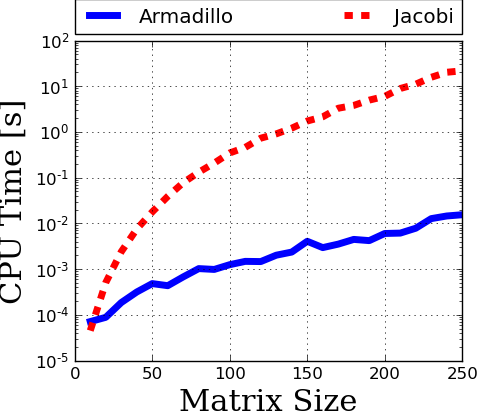
\includegraphics[keepaspectratio,height=7cm, width=8cm]{arma_vs_jacobi.png}
  \caption{CPU time in seconds for solving the buckling beam eigenvalue problem for different matrix sizes using Jacobi rotation and Armadillo.}
   \label{arma_vs_jacobi}
\end{figure}

The three first eigenvectors of the buckling beam problem are shown in Fig. \ref{beam_eigvec}. Here, the number of discretization points (or matrix size) are fixed to be $250$ and the solution from the Jacobi rotation method, Armadillo, and its corresponding analytical solution are presented. It is pertinent to notice the match between the analytical and the numerical solution. Physically, the eigenvectors of the buckling beam problem illustrate the different modes of vibration (i.e., standing waves) of the beam. 

\begin{figure}[H]
  \centering
  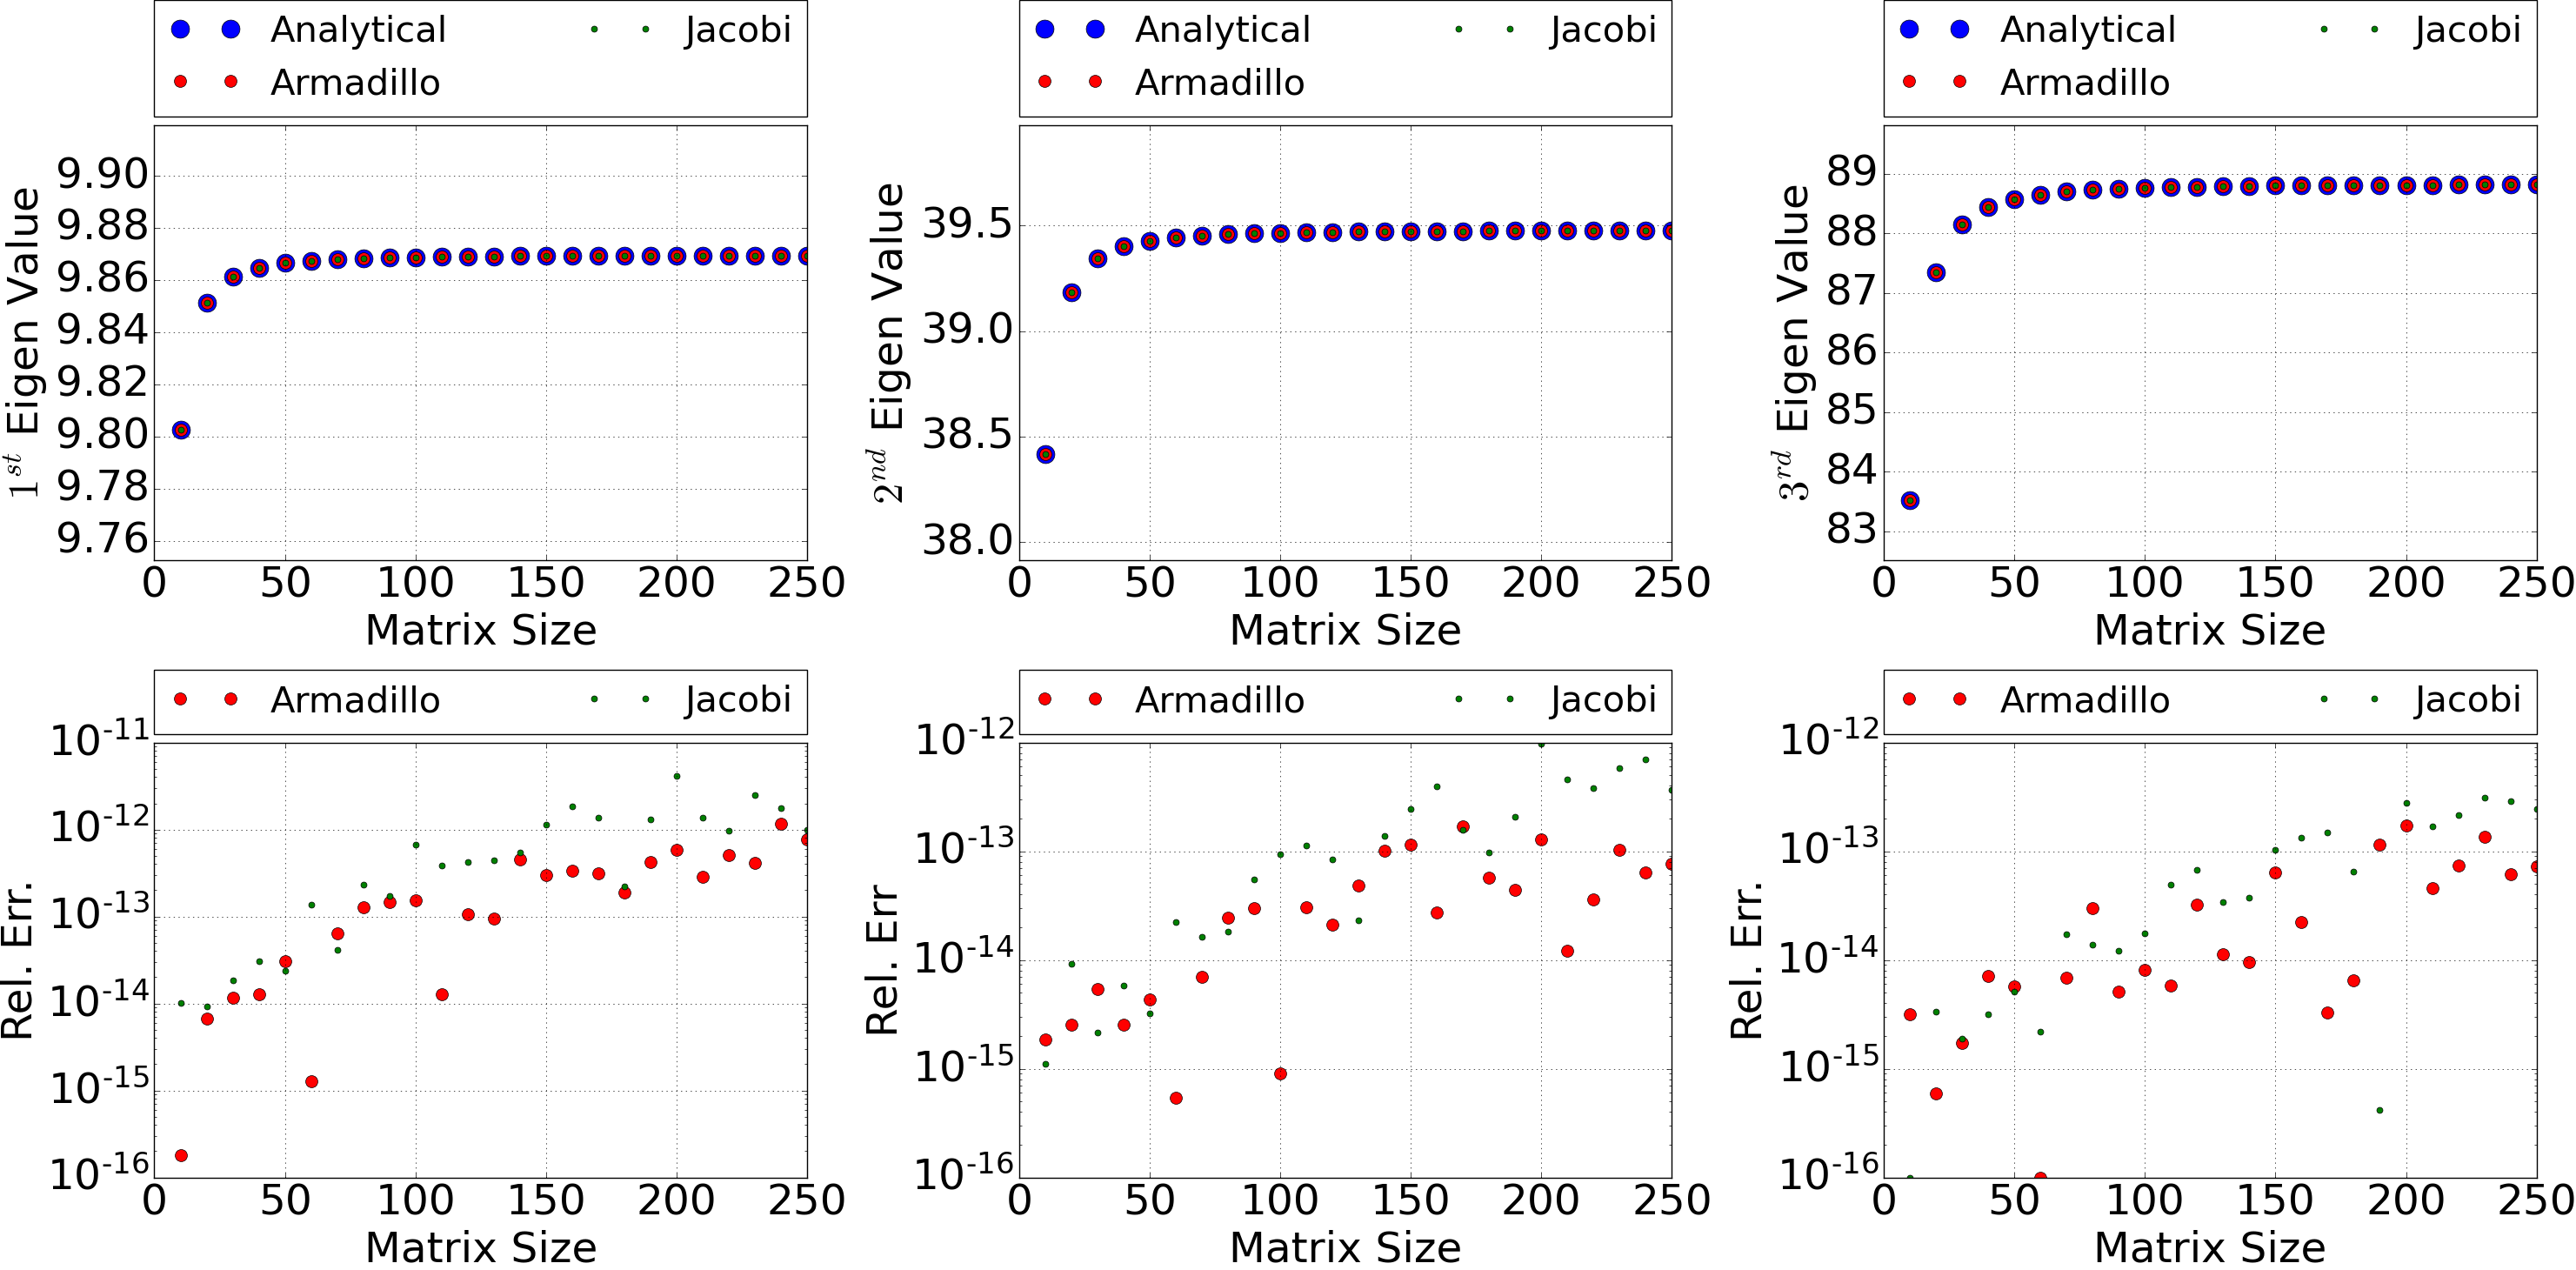
\includegraphics[keepaspectratio,height=8cm, width=12cm]{beam_eigval.png}
  \caption{The first three eigenvalues of the buckling beam problem computed using Jacobi rotation, Armadillo and its corresponding analytical solution. The relative error of the Jacobi and Armadillo method is shown in the bottom row.}
   \label{beam_eigval}
\end{figure}
\begin{figure}[H]
  \centering
  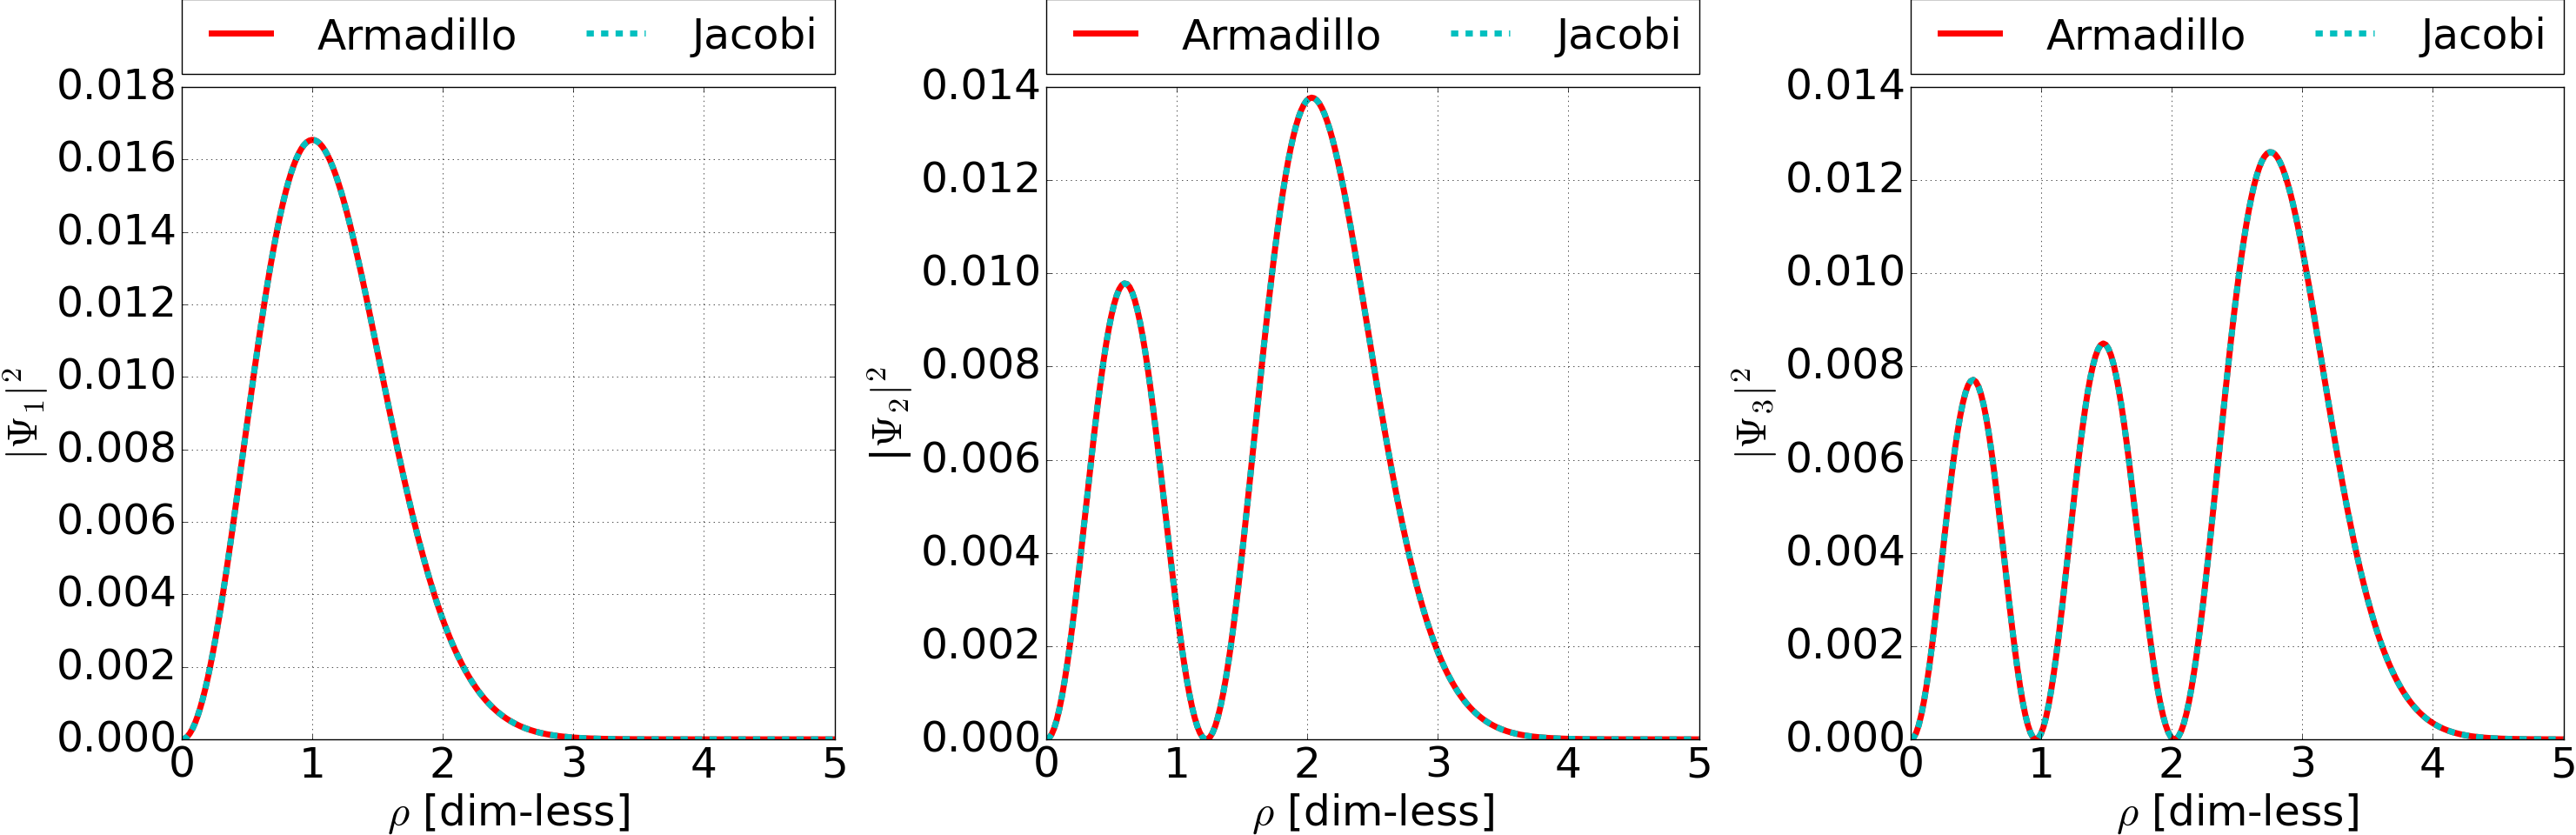
\includegraphics[keepaspectratio,height=4cm, width=12cm]{beam_eigvec.png}
  \caption{The first three eigen vectors of the buckling beam problem computed using Jacobi rotation, Armadillo and its corresponding analytical solution.}
   \label{beam_eigvec}
\end{figure}

\subsection{Single electron in a harmonic oscillator potential}
Numerically solving the problem of a single electron in a harmonic oscillator potential requires an optimization for finding a suitable $\rho_{max}$ value. In addition, since we have an analytical solutions for the eigenvalues, we can check the number of integration points (discretization points) required to reach the analytical solutions with an acceptable relative error. After searching $\rho_{max}$ within the range between $1$ and $10$, and the number of discretization points ($N$) between $10$ and $250$, we found the smallest relative error when $\rho_{max} = 5$ and $N=250$. The first three eigenvalues as a function of the discretization points is shown in Fig. \ref{1el_eigval} (top row) for the three different ways of solving the problem. The relative error for the Jacobi method and Armadillo are shown in Fig. \ref{1el_eigval} (bottom row). The relative error for the first eigenvalue when using $N=250$ is $\sim10^{-4.5}$, for the second $\sim10^{-4}$, and the third $\sim10^{-4}$. Compared to the buckling beam problem, solving the single electron problem using numerical eigenvalue problem solvers is less precise. 

We calculated the radial probability density of the electron for the first three eigenvalues (cf. Fig. \ref{1el_eigvec}). As the eigenvalues gets larger (i.e., higher energy levels) the probability of finding the electron also shifts away from the origin. 

\begin{figure}[H]
  \centering
  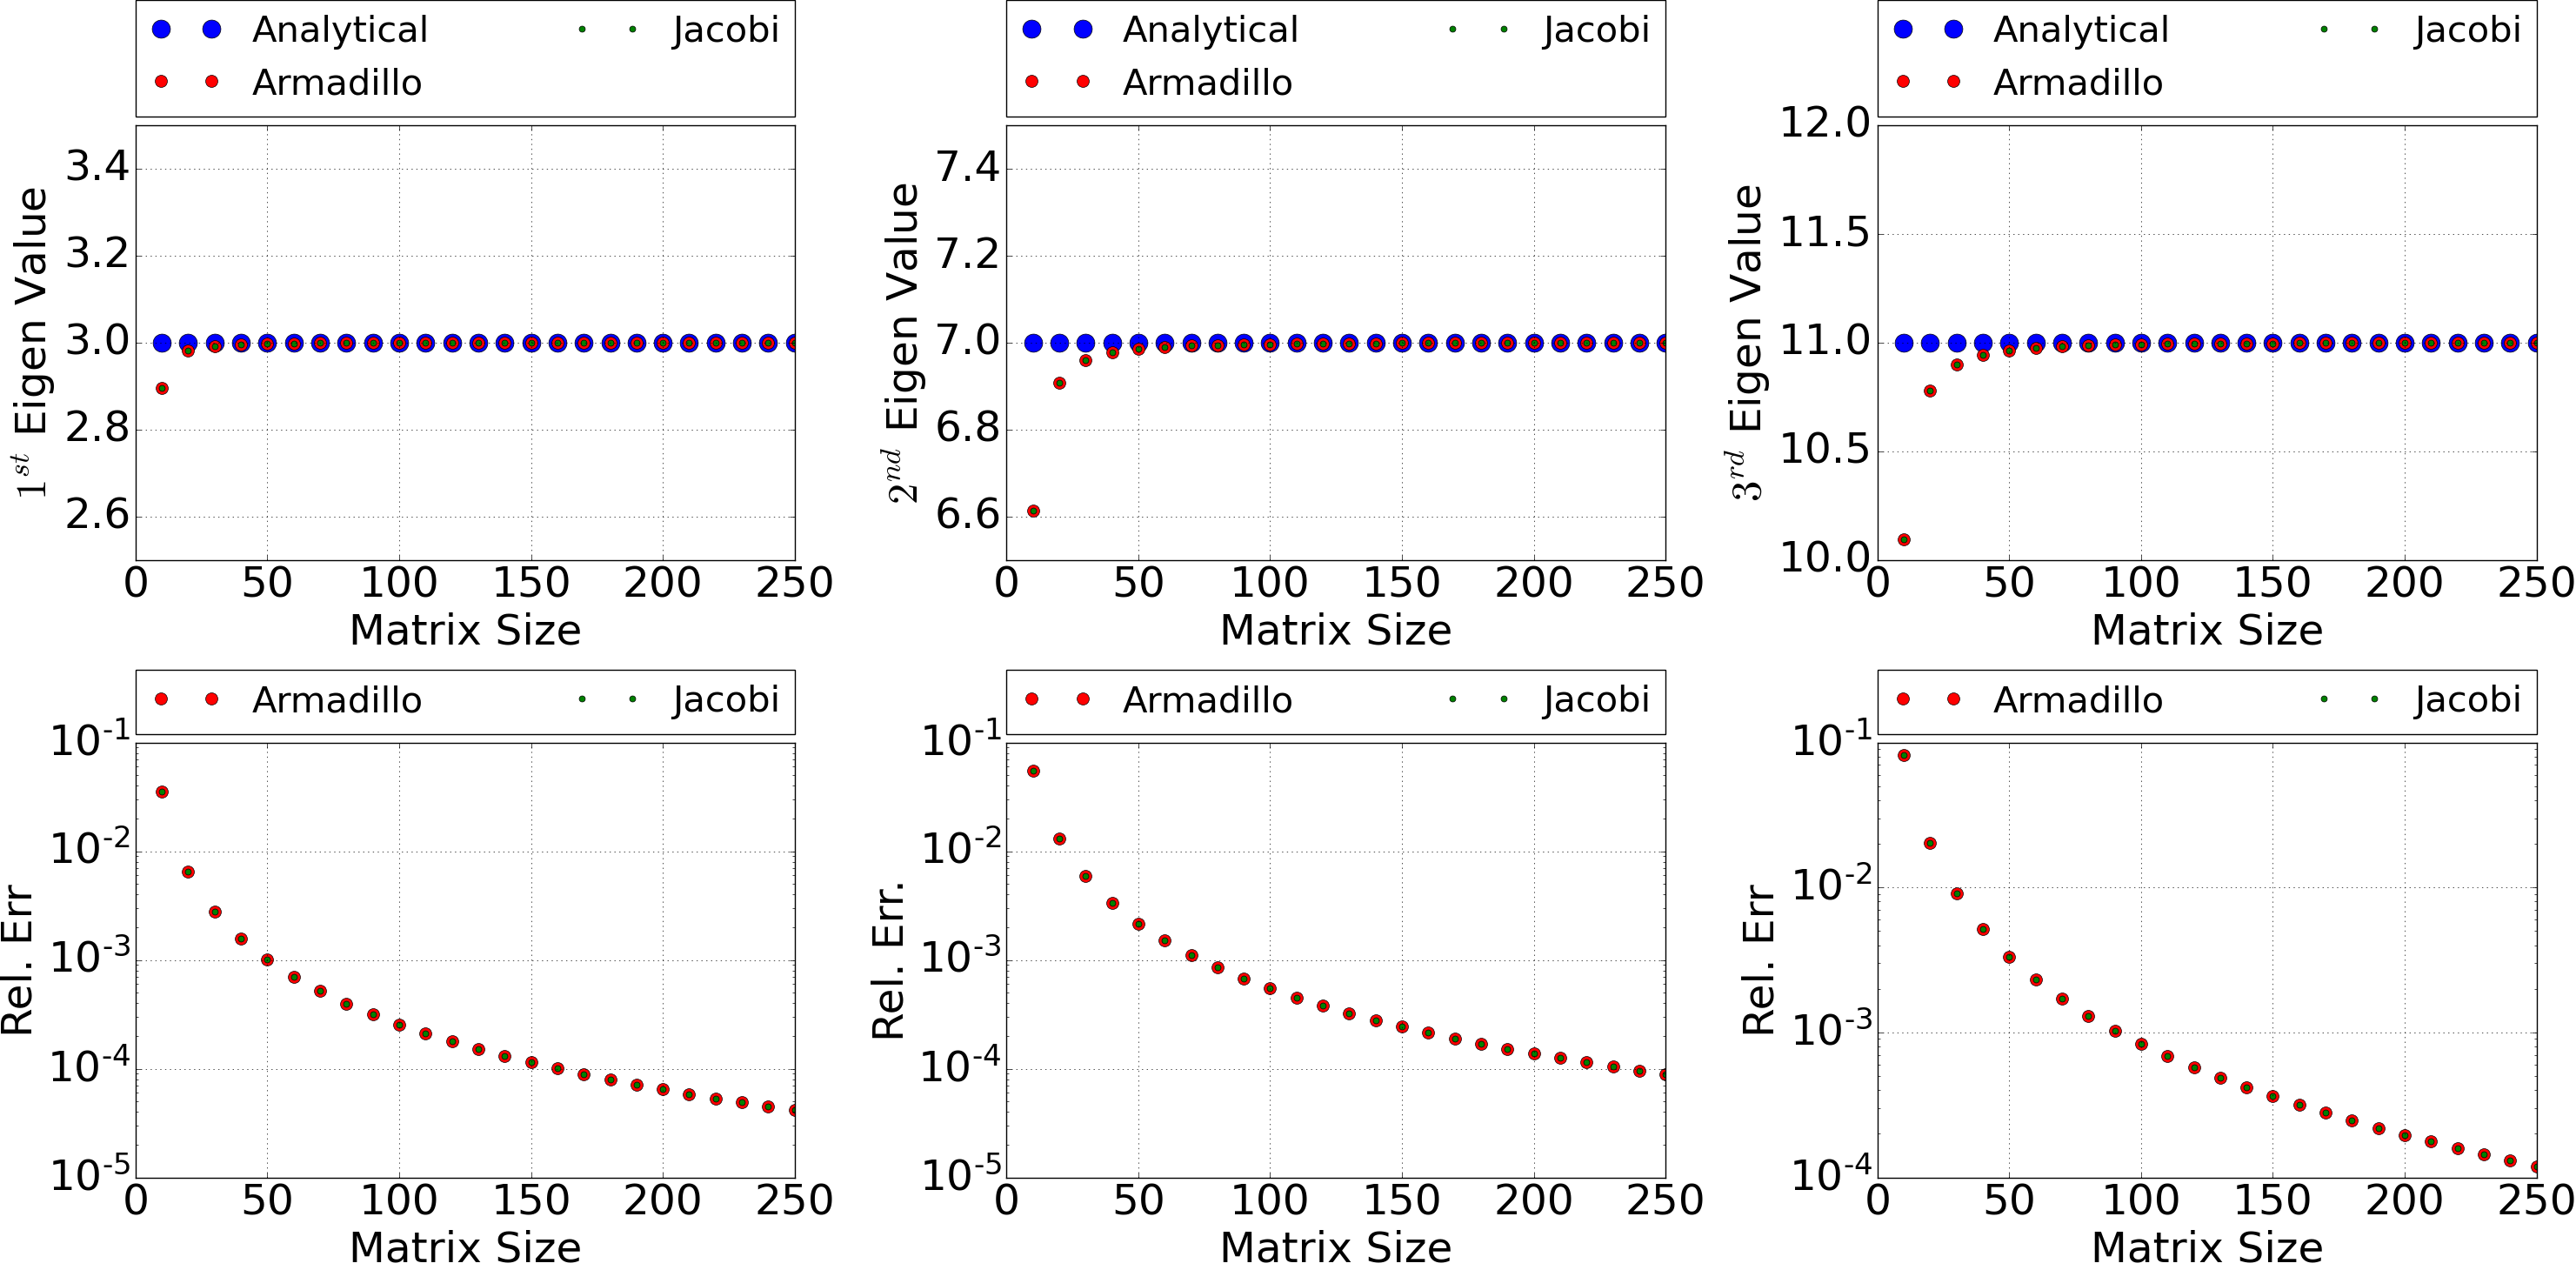
\includegraphics[keepaspectratio,height=10cm, width=12cm]{1el_eigval.png}
  \caption{The first three eigenvalues of the single electron problem computed using Jacobi rotation, Armadillo and its corresponding analytical solution. The relative error of the Jacobi and Armadillo method is shown in the bottom row. Notice we have used $\rho_{max}=5$}.
   \label{1el_eigval}
\end{figure}
\begin{figure}[H]
  \centering
  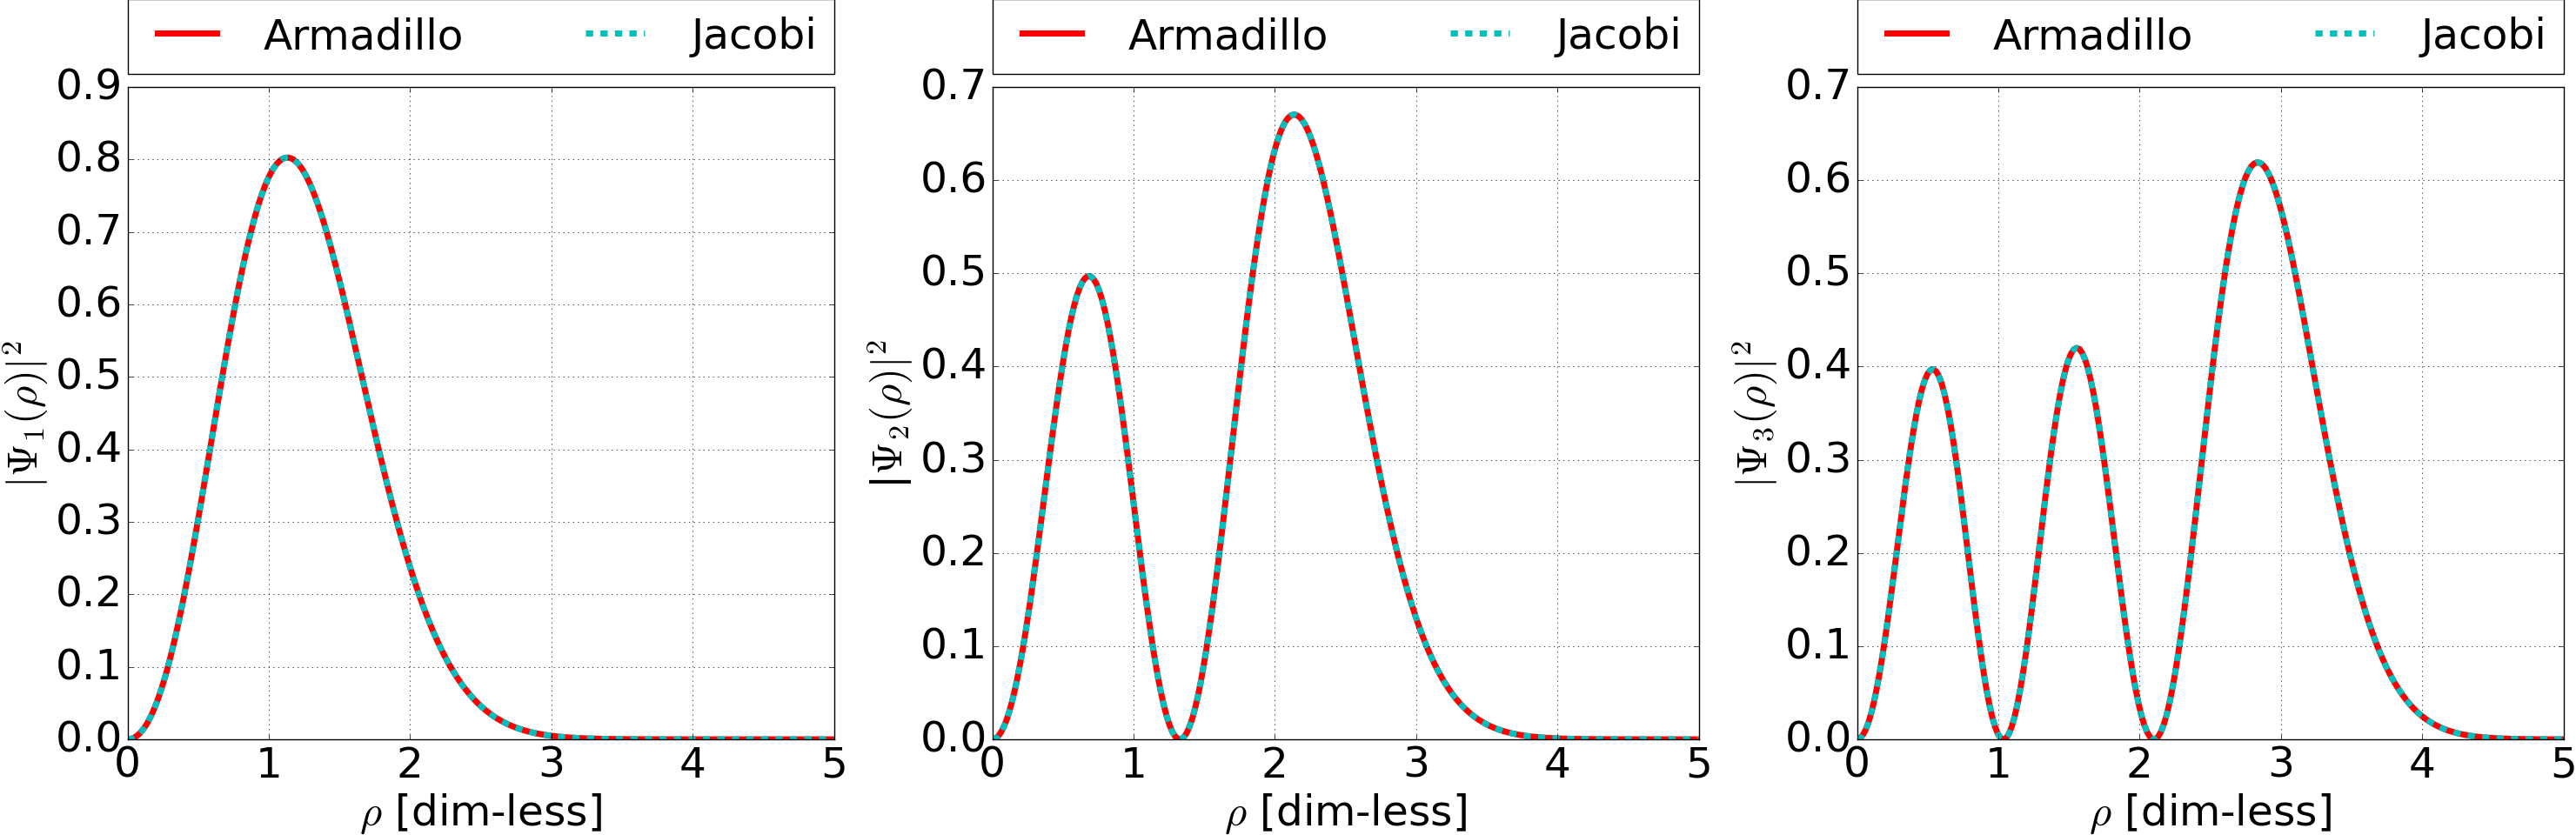
\includegraphics[keepaspectratio,height=10cm, width=12cm]{1el_eigvec.png}
  \caption{The first three radial probability densities of the single electron problem computed using Jacobi rotation and Armadillo.}
   \label{1el_eigvec}
\end{figure}
\subsection{Two electrons in a harmonic oscillator potential}
We now consider two electrons in a harmonic potential with and without Coulomb interactions. For the two electrons with Coulomb intraction case the eigenvalue problem presented in section \ref{2elec} has analytical solution \cite{PhysRevA.48.3561} for some specific values of $\omega_r$. We compared our Jacobi algorithm solution with that of the analytical and computed relative errors (cf. Table \ref{table:eigenvalues}). All the numerical calculations were performed using $250$ integration points. Here, it is pertinent to notice that as the oscillator parameter $\omega_r$ decreases the value of $\rho_{max}$ needed to be increased to mach the analytical solution.

\begin{table}[H]
\caption{The ground state eigenvalues for the two interacting electrons computed using analytical and Jacobi rotation methods. different values of $\omega_r$.\\}
\begin{center}
  \begin{tabular}{|l | l |l |l |l| }
  \hline
    $\omega_r$  & $\rho_{max}$ & Analytical & Jacobi & Relative Error  \\[0.10cm]\hline\hline
     $0.25$     & $10$ & $1.25$     & $1.2499$  & $1\times10^{-04}$\\[0.10cm]
     $0.05$     & $20$ & $0.35$     & $0.3499$  & $2.6\times10^{-05}$\\[0.10cm]
     $0.01827$  & $30$ & $0.1644$   & $0.16444$ &$2.99\times10^{-04}$\\[0.10cm]
     
     \hline
  \end{tabular}
     \label{table:eigenvalues}
\end{center}
\end{table}

The probability density for the ground state of the two interacting electrons system is shown in Fig. \ref{2el_eigvec} for the oscillator parameters $\omega_r = 0.01, 0.5, 1,$ and $5$. Here, we can see the peak of the probability density function move closer to zero when $\omega_r$ gets larger. This is due to the fact that the oscillator potential gets wider when $\omega_r$ gets smaller and this allows the two electrons to move further away from each other.

To investigate the effect of the Coulomb interaction on the two electrons, we computed the probability density function for the interacting and non-interacting two electrons with $\omega_r = 1$ and $0.5$ (see Fig. \ref{2el_eigvec_interact}). Both the interacting and non-interacting cases show the probability density functions peak shift to larger distances between the two electrons when $\omega_r$ gets smaller. Moreover, we also notice a counter intuitive behaviour that the probability density function for interacting electrons with smaller $\omega_r$ appear further away from each other than its corresponding non-interacting case. This behaviour is due to the infinite range of the Coulomb interaction and the fact that the harmonic oscillator energy reduces to zeros as $\omega_r$ approaches to zero.

\begin{figure}[H]
  \centering
  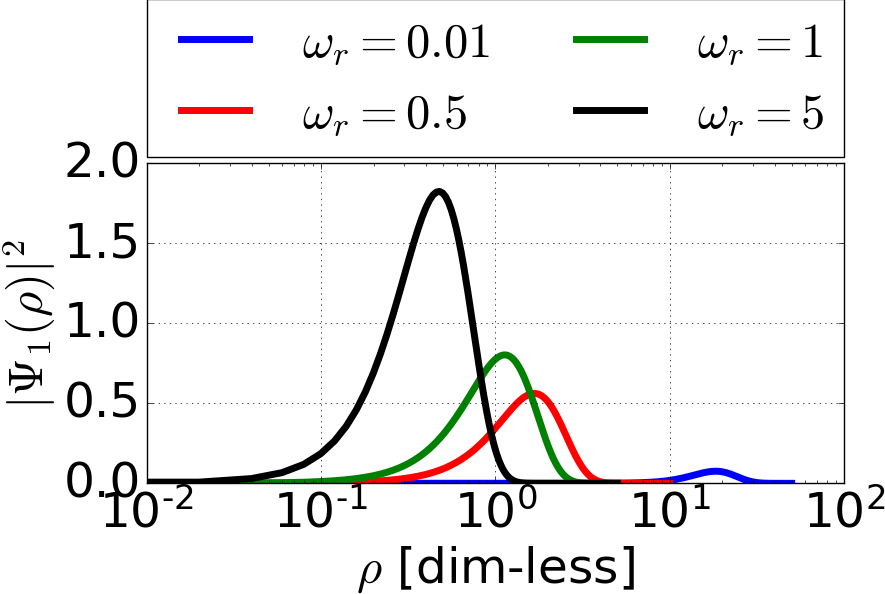
\includegraphics[keepaspectratio,height=10cm, width=12cm]{2el_eigvec.png}
  \caption{The radial probability densities of the ground state of the two interacting electrons in a harmonic oscillator potential for different values of $\omega_r$. Notice $\rho$ is the scaled relative distance between the two electrons.}
   \label{2el_eigvec}
\end{figure}
\begin{figure}[H]
  \centering
  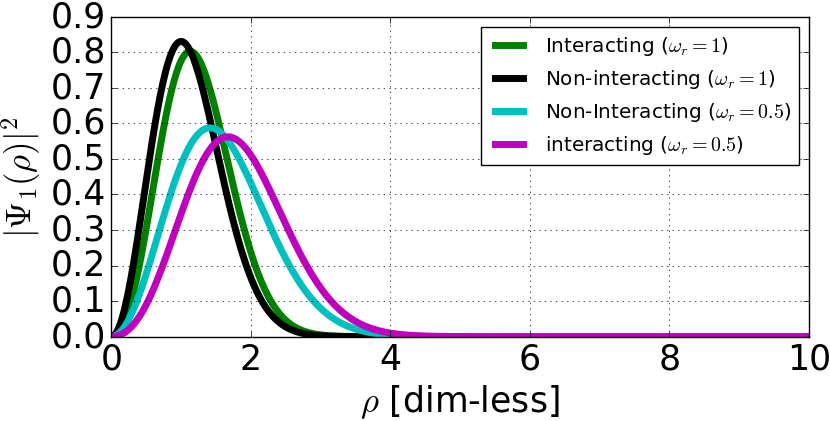
\includegraphics[keepaspectratio,height=10cm, width=12cm]{2el_eigvec_interact.png}
%   \caption{The radial probability densities of the ground state of the two interacting and non-interacting electrons in a harmonic oscillator potential for $\omega_r=1$ and $\omega_r=0.5$.}
  \caption{The radial probability densities of the ground state of the two interacting and non-interacting electrons in a harmonic oscillator potential for $\omega_r=1$ and $\omega_r=0.5$. We see that when the potential of the well gets larger (steered by setting $\omega_r$ smaller) the Columb interaction, 1/$\rho$, effectivly is forcing the electrons further away from the center compared to the non-interacting case.}
   \label{2el_eigvec_interact}
\end{figure}
\section{Discussion}
Jacobi rotation algorithm for solving larger size eigenvalue problems is inefficient. From Fig. \ref{N_vs_Rotation} we have seen that the number of similarity transformations performed by the Jacobi algorithm depends on the number of gird points (or size of the matrix $n$). This dependence was shown to be quadratic ($n^2$) in our case. We have also seen the number of FLOPs per iteration go as $n^2$, therefore the total number of FLOPs for the Jacobi algorithm is $\mathcal{O}(n^4)$. 

% $n^2$, therefore the total number of FLOPs for the Jacobi algorithm is $\mathcal{O}(n^4)$. 

The three eigenvalue problems we consider in this project results in a tridiagonal matrix eigenvalue problem. However, we used the Jacobi rotation algorithm, which is designed for solving small size dense matrices. Therefore, the comparison of Jacobi's algorithm with that of Armadillo's implementation (which identifies the matrix type and use the most efficient method) shows how inefficient Jacobi's algorithm is for larger size matrices.

\section{Conclusion}
The Jacobi method, despite being inefficient compared to Armadillo's implementation, managed to generate the correct eigenvalues and eigenvectors for the buckling beam and quantum dots problems considered in this project. 

The accuracy of the Jacobi method is evaluated by comparing the resulting eigenvalues and eigenvectors with the corresponding exact analytical solutions. For a matrix size of $250\times 250$, the relative error for the buckling beam problem is in the order of $\sim10^{-11}$. However, for the quantum dot problems with one and two electrons, the relative error is in the order of $\sim10^{-4}$. The loss of accuracy in the later case is due to the fact that we have approximated $\rho_{max} = \infty$ with a finite value.

The eigenvalues and eigenvectors of the buckling beam provide physical insight about the energy and mode of vibration, respectively. For the quantum dot examples, the eigenvalues are related to the different energy states of the electron(s) while the eigenvectors represent the wavefunctions, which can be squared to provide the probability densities.

%\bibliographystyle{plain}
%\bibliographystyle{siam}
\bibliography{sample}
\bibliographystyle{IEEEtran}

\begin{appendix}
\section{Orthogonality Preservation}
Here, we proof the preservation of orthogonality and dot product after similarity transformations. Similarity transformations are unitary transformations. Now, we consider an orthogonal basis vector $\mathbf{v}_i\in\mathbf{R}^{n}$ and an unitary
transformation matrix $\mathbf{U}\in\mathbf{R}^{n\times n}$. Defining $\mathbf{w}_i=\mathbf{U}\mathbf{v}_i$, the dot product can
be computed as
\begin{align*}
	\mathbf{w}_j^T\cdot\mathbf{w}_i&=(\mathbf{U}\mathbf{v}_j)^T\cdot (\mathbf{U}\mathbf{v}_i)=\mathbf{U}^T\mathbf{v}_j^T\cdot \mathbf{U}\mathbf{v}_i=\mathbf{U}^T\mathbf{U}\mathbf{v}_j^T\cdot\mathbf{v}_i \\
&=\mathbf{U}^{-1}\mathbf{U}\mathbf{v}_j^T\cdot\mathbf{v}_i=\mathbf{I}\mathbf{v}_j^T\cdot\mathbf{v}_i=\delta_{ij}
\end{align*}


where $\mathbf{I}\in\mathbb{R}^{n\times n}$ is the identity matrix and the third last equality holds due to $\mathbf{U}^T=\mathbf{U}^{-1}$ for orthogonal matrices.

\section{Similarity transformations}

If $n\times n$ matrices $\mbox{\boldmath$A$}$ and $\mbox{\boldmath$B$}$ are similar, then they have the same characteristic polynombial and hence the same eigenvalues.

\label{sim_tran}
\begin{proof}:
% \begin{center}
% \normalsize
% \small
\begin{adjustwidth}{20pt}{0pt}

\footnotesize


\mbox{\boldmath$B$}
\quad\quad\quad \,\,\,\,\,= \mbox{\boldmath$G^{-1}AG$} 

\mbox{\boldmath$B$} -
$\mathbin{\textcolor{red}{\lambda\mbox{\boldmath$I$} }}$
\,\,\,\,\quad = \mbox{\boldmath$G^{-1}AG$}  - $\mathbin{\textcolor{red}{\lambda\mbox{\boldmath$G^{-1}G$} }}$
,\quad\quad\quad\quad since \mbox{\boldmath$I$} = \mbox{\boldmath$G^{-1}G$}, also note $\lambda$ is a scalar

\quad\quad\quad\quad\quad  =
\mbox{\boldmath$G^{-1}AG -$}
$\mathbin{\textcolor{red}{\lambda}}$\mbox{\boldmath$G^{-1}G$}



\quad\quad\quad\quad\quad  =
$\mathbin{\textcolor{blue}{\mbox{\boldmath$G^{-1}$} }}$
 \mbox{\boldmath$AG - $}
$\mathbin{\textcolor{blue}{\mbox{\boldmath$G^{-1}$} }}$
$\mathbin{\textcolor{red}{\lambda}}$\mbox{\boldmath$G$}

\quad\quad\quad\quad\quad=
$\mathbin{\textcolor{blue}{\mbox{\boldmath$G^{-1}$} }}$
$\mbox{\boldmath$(A$}$$\mathbin{\textcolor{green}{\mbox{\boldmath$G - $} }}$
$\lambda$$\mathbin{\textcolor{green}{\mbox{\boldmath$G$} }}$$\mbox{\boldmath$)$}$

\mbox{\boldmath$B-$}$\lambda$\mbox{\boldmath$I$} \,\,\,\,\,\quad=
$\mbox{\boldmath$G^{-1}(A - $}$$\lambda$$\mbox{\boldmath$I)$}$$\mathbin{\textcolor{green}{\mbox{\boldmath$G$} }}$
\end{adjustwidth}
% \mbox{\boldmath$B-$}$\lambda$\mbox{\boldmath$I$} \,\,\,\,= \mbox{\boldmath$P^{-1}(A-$}$\lambda$\mbox{\boldmath$I)P$}

Now we use a rule for determinates which is stating that:
\begin{adjustwidth}{20pt}{50pt}
\footnotesize
det$\mbox{\boldmath$(AB)$}$\,\,\,\, = det$\mbox{\boldmath$(A)$}$*det$\mbox{\boldmath$(B)$}$
\end{adjustwidth}
We then have
\begin{adjustwidth}{20pt}{50pt}
\footnotesize

det$\mbox{\boldmath$(B$}$-$\lambda\mbox{\boldmath$I)$}$ = det\mbox{\boldmath$($}$\mathbin{\textcolor{red}{\mbox{\boldmath$G^{-1}$} }}$$\mbox{\boldmath$[A-$}$$\lambda$\mbox{\boldmath$I]$}$\mathbin{\textcolor{red}{\mbox{\boldmath$G$} }}$\mbox{\boldmath$)$}


\quad\quad\quad\quad\quad=
det\mbox{\boldmath$($}$\mathbin{\textcolor{red}{\mbox{\boldmath$G^{-1}$} }}$\mbox{\boldmath$)$}*det\mbox{\boldmath$(A - $}$\lambda$\mbox{\boldmath$I)$}*det\mbox{\boldmath$($}$\mathbin{\textcolor{red}{\mbox{\boldmath$G$} }}$\mbox{\boldmath$)$}


\quad\quad\quad\quad\quad= 
det\mbox{\boldmath$($}$\mathbin{\textcolor{red}{\mbox{\boldmath$G^{-1}$} }}$\mbox{\boldmath$)$}
*det\mbox{\boldmath$($}$\mathbin{\textcolor{red}{\mbox{\boldmath$G$} }}$\mbox{\boldmath$)$}*det\mbox{\boldmath$(A-$}$\lambda$\mbox{\boldmath$)$}



\quad\quad\quad\quad\quad=
det\mbox{\boldmath$($}$\mathbin{\textcolor{red}{\mbox{\boldmath$G^{-1}G$} }}$\mbox{\boldmath$)$}*det\mbox{\boldmath$(A-$}$\lambda$\mbox{\boldmath$)$}, \quad\quad where det\mbox{\boldmath$($}$\mathbin{\textcolor{red}{\mbox{\boldmath$G^{-1}G$} }}$\mbox{\boldmath$)$} = det\mbox{\boldmath$(I)$}

det$\mbox{\boldmath$(B$}$-$\lambda\mbox{\boldmath$I)$}$ = 
det$\mbox{\boldmath$(A$}$-$\lambda\mbox{\boldmath$I)$}$ 
\end{adjustwidth}
\end{proof}



\end{appendix}
\end{document}
